\section{Termination} \label{termination} %do writing new stuff in the morning, fixing in the afternoon.
%reset in case acronyms are cited previously, this is their main paragraph and the acronym needs to be in long form.
\glsreset{cpf}
\glsreset{nns}
After its synthesis and maturation are complete, the nascent RNA molecule must be released from the DNA template, and the elongation complex must be disassembled and its components recycled.
In \cer{}, transcription termination is enacted by several widely different mechanisms.
Two predominating pathways terminate the vast majority of transcripts generated by \acrlong{pol2}: the \gls{cpf} pathway and the \gls{nns}  pathway. 
Both these mechanisms rely on short sequences on the nascent RNA---coupled with specific modifications on the \gls{ctd} of \gls{pol2}---to recruit specific factors and enact the disassembly of the elongation complex and the release of the transcript in the nucleus.

Owing to the imperfection of biological systems, the cell has evolved several additional non-canonical systems to terminate transcription. Should \gls{cpf} or \gls{nns} fail in their tasks, at least one transcription factor is able to act as road-block for \gls{pol2} and bring about transcription termination. Additionally, the \gls{sns} processing factor Rnt1 is able to act as an emergency termination factor in certain circumstances. \TODO{check correctness and expand pls.}

Transcription termination is also strictly intertwined with some steps of 3' end processing and maturation. 
The \gls{cpf} complex couples termination with a polyadenylation step and export competence of the RNA was shown to require this termination mechanism. \TODO{check and expand, again} 




\subsection{The CPF-CF pathway}
The \gls{cpf} pathway was the first termination mechanism described in \cer{} because of its association with the termination of protein-coding genes\TODO{ref?}\TODO{put section label in footnote}\footnote{Its activity can extend to certain kinds of non-coding transcripts as well (see SECTIONLABEL for details)}. 
\gls{cpf} termination is unique as it results in cleavage of the nascent RNA before termination occurs.
The site of cleavage is specified through sequence elements present on the nascent RNA and plays an important role in kickstarting the termination reaction.

There exist some controversy about how \gls{cpf} termination mechanistically occurs.
The literature proposes for two models that explain termination through the \gls{cpf} pathway.
The allosteric model argues that transcription through the cleavage site leads to conformational changes in the elongation complex, leading to destabilization of the complex and eventually termination.
On the other hand, the torpedo model posits that after cleavage, the uncapped 5' end of the polymerase-associated transcript is attacked by exonuclease Rat1, leading to the dismantling of the complex through destabilization of the ternary complex once Rat1 catches up with the polymerase.

Regardless of the model, the main actor of this termination mechanism is the \gls{cpf} complex, a large assembly of modular sub-complexes that act in concert to execute all the required steps. 
This complexity makes \gls{cpf} the most reliable, efficient, and precise termination mechanism in \cer{}.

\subsubsection{Recruitment and assembly}
\TODO{figure}
Recruitment and initial assembly of the \gls{cpf} complex onto the nascent RNA is promoted by two mechanisms: interaction with specific sequences elements, and interaction with the polymerase \gls{ctd}.

A key component of the \gls{cpf} complex, Pcf11, contains a peptide sequence able to recognize the \gls{ctd}. This \gls{cid} is able to specifically recognize the \sert{}-phosphorylated version of the heptapeptide.
Given the nature of this \gls{ctd} modification---which is confined to the later stages of transcription---density of the \gls{cpf} complex around the polymerase is selectively increased where the complex is more likely to be needed for termination (i.e. at the 3' end of transcription units), facilitating the eventual binding of \gls{cpf} to the sequence elements on the nascent RNA.

Unlike in human, where the cleavage site is defined by a single highly conserved hexanucleotide sequence on the nascent RNA, Yeast \gls{cpf} complex recognizes a number of degenerate short sequences.
Two sub-complexes of \gls{cpf}, \gls{cf1a} and \gls{cf1b}, are responsible for the recognition of these sequences.
In particular, Rna15 and Hrp1 (components of \gls{cf1a} and \gls{cf1b} respectively) directly bind the nascent RNA.
Associated factors Rna14 and Pcf11 contribute to the assembly of the whole complex by interacting with \gls{pol2} and forming a scaffold that serves to tether the catalytic portion of the \gls{cpf} complex to the cleavage site.

The bulk of the catalytic activity of the \gls{cpf} complex is contained in the \gls{cpfa} sub-complex.
\gls{cpfa} directly contacts the cleavage site with its Ysh1 subunit and is responsible of the cleavage of the nascent RNA, one of the events that is thought to kickstart the termination reaction.
\gls{cpfa} also coordinates the polyadenylation reaction through the subunits Yth1 and Fip1. 
These factors recruit and tether the poly(A) polymerase Pap1 to the complex, which will begin catalyzing the addition of a poly(A) tail after the transcript has been cleaved.

\subsubsection{The torpedo model}

After cleavage and release of the nascent RNA, the elongation complex has successfully accomplished its job in the transcriptional process and is ready to be disassembled.
The ``torpedo" model is one of the two main mechanistic models that describes the process by which the \gls{tec} is removed from the DNA template.
According to this model, cleavage represents the main termination signal for the \gls{cpf} complex, as it leaves an uncapped 5'-P on the transcript associated with the still transcribing elongation complex.
These unprotected 5' is the substrate of \FtoT{} exonucleases, a class of enzymes that are known to progressively degrade RNA polypeptides.
The \FtoT{} exonuclease Rat1 was discovered to be associated with the \gls{cpf} complex and is thought to attack the 5' moiety of the \gls{pol2}-associated transcript, starting a processivity race with \gls{pol2}.
Upon winning the race, Rat1 would destabilize the structure of the ternary complex within the polymerase, causing it to break apart and detach from the DNA template.

There are several lines of evidence that support this model for \gls{cpf} transcription termination.
Both Rat1 and its human homolog Xrn2 exhibit termination defects in model cases when mutated \citep{kim:2004:yeast, west:2004:human}.
Furthermore, Rat1 and its co-factor Rtt103 were found to be strongly associated with the 3' end of genes and in physical association with the \gls{cpf} complex \citep{kim:2004:yeast,luo:2006:role}, supporting the idea of a functional recruitment to zones of active transcription termination.
Homology studies found that homologs of Rtt103 in both humans and \cele{} have roles in transcription termination\citep{morales:2014:kub5hera, cui:2008:genes}.
Finally, recent mechanistic studies \invivo{} have demonstrated the kinetic competition between Rat1 and the elongation complex. By employing mutant polymerases that elongate faster or slower than the wild type version, the authors were able to show that slower polymerases result in earlier termination, consistent with the notion that Rat1 needs to physically catch up with the polymerase in order to elicit termination\citep{fong:2015:effects}.

At the same time, several reports argue against the torpedo model as sole effector of transcription termination.
\emph{In vitro} studies were unable to reproduce the termination effect observed \invivo{} using only Rat1 \citep{dengl:2009:torpedo}. More recent ventures re-attempted the \invitro{} approach with limited success \citep{park:2015:unraveling}, but managed to demostrate that Rat1 is able to terminate polymerases that are destabilized by nucleotide misincorporation.
Several additional mechanistic studies showed that the exonucleolytic activity of Rat1 is unable to mediate the release of the polymerase from the template \citep{luo:2006:role, pearson:2013:dismantling}.
Moreover, termination defects caused by Rat1 mutants were not associated with stabilization of the \gls{pol2}-associated transcript, arguing against the model.
Finally, recent genome-wide studies were unsuccessful in detecting a widespread effect of Rat1 human homolog (Xrn2) in transcription termination\citep{nojima:2015:mammalian}.


\subsubsection{The allosteric model}

The torpedo model relies exclusively on cleavage of the RNA as a trigger for transcription termination.
An alternative model argues that cleavage is a dispensable signal, and that termination can happen independently of this step.
This ``allosteric" model posits that after transcription of the cleavage site, \gls{pol2} loses a lot of factors that qualify the elongation complex as such.
The loss of these ``anti-terminator" factors---components of the elongation complex that would prevent termination from happening---would trigger conformational changes, destabilize the polymerase, and allow components of the \gls{cpf} complex itself to elicit the disassembly of \gls{pol2} from the template.

Several studies support this model. 
\gls{pol2} was shown to lose a number of associated elongation factors after reaching the 3' end \citep{kim:2004:transitions}.
In addition, the component of the \gls{cpf} complex Pcf11 was shown to be able to terminate the polymerase \invitro{} by binding the nascent RNA and the \sert{}-phosphorylated moiety of \gls{pol2} \citep{zhang:2005:ctddependent}.
Ulterior support to this last study was provided by the same authors two years later, when they discovered that Pcf11 is able to perform the same feat in drosophila\citep{zhang:2006:pcf11}.
Finally, a very recent study published on Molecular Cell was able to reconstitute transcription termination in an \invitro{} system in the absence of cleavage\citep{zhang:2015:polya}.

\subsubsection{A unified view of CPF-CF transcription termination}

As evidence for and against the two models piles up, a unified view that combines elements of both torpedo and allosteric model is taking shape.
While the effect of Rat1 on transcription termination (of at least some transcripts) is established, its role as main effector of \gls{cpf} termination has been repeatedly called into question.
Several studies have now described interdependencies between Rat1 and other subunits of the \gls{cpf} complex---notably Pcf11---and the perceived nature of Rat1 is shifting towards that of a molecular effector  that is integrated into a larger system.
Moreover, proof of principle that termination is possible without cleavage has been recently provided---albeit \invitro{}---casting further doubt on the role of Rat1 and its exonucleolytic activity on transcription termination.

\begin{figure}[ht]

\centering
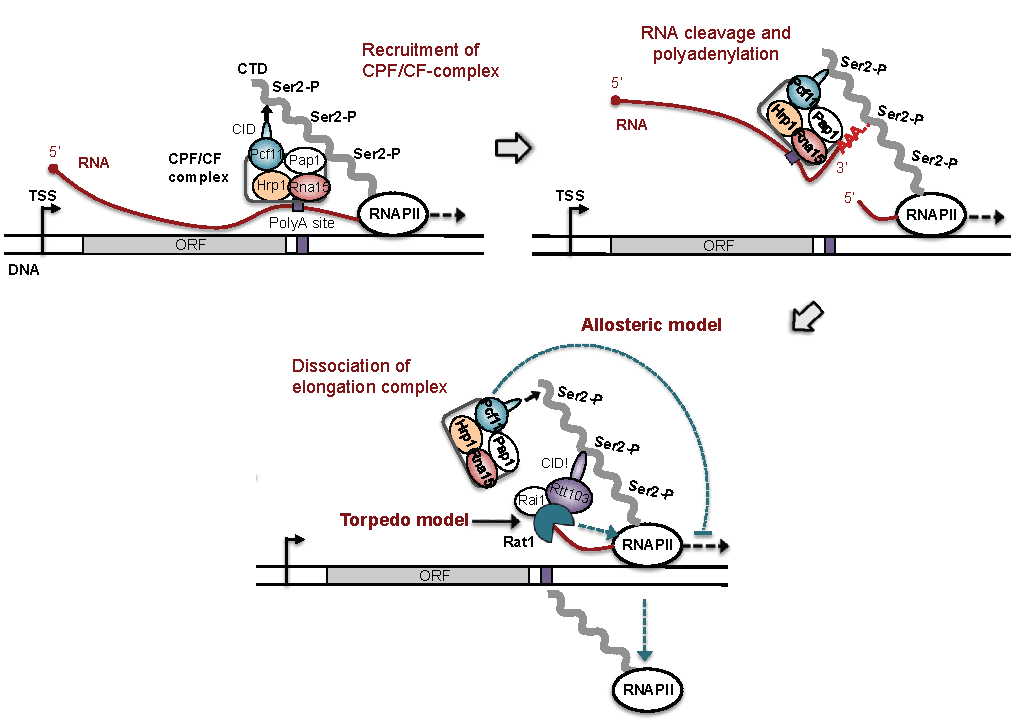
\includegraphics[width=\textwidth]{figures/introduction/cpf}
\caption[Mechanism of CPF-CF termination]{Overview of the main mechanistic step that lead to CPF-CF termination. The complex is recruited thanks to CTD phosphorylation and binding sites on the RNA. The transcript is then cleaved and the elongation complex terminated in accordance with the torpedo or allosteric model.}
\label{fig:cpfTermination}

\end{figure}

Despite recent advances and the rise of a unified model for transcription termination, mechanistic details on the termination reaction and what prompts it are still sorely lacking.



\subsection{The NNS pathway}

\gls{nns} dependent transcription termination is the second wide-spread termination mechanism in \cer{}.
It sets itself apart from \gls{cpf} termination in a number of ways.
First and foremost, it relies on a completely different---and much smaller---set of proteins: the two RNA binding proteins Nrd1 and Nab3, together with the RNA-DNA helicase Sen1.
Because of the different molecular effectors, the termination mechanism---although still not fully elucidated---is appreciably different.
It does not result in cleavage of the RNA transcript, but instead it is the disassembly of the elongation itself that mediates the release of the transcript. 
As a consequence, the 3' end of the terminated transcript coincide with the termination site on DNA, making \gls{nns} termination substantially less precise than \gls{cpf}.
The \gls{nns} complex also recruits a completely different set of 3' end processing and maturation factors collectively known as \gls{tramp} (\glsdesc{tramp}), which drives post-transcriptional polyadenylation and leads to trimming or complete degradation of the transcript by the nuclear exosome. 

\gls{nns} termination operates mainly on non-coding RNAs and acts in the very early stages of transcription.
Despite not being directly involved in the termination of protein-coding genes, it can play a role in the regulation of gene expression by acting as an attenuator (i.e. terminating some transcription events very early in the transcription cycle, preventing them from coming to completion.) or otherwise modulating the transcription of nearby non-coding RNAs.


\subsubsection{The NNS complex}

The main molecular effectors of the \gls{nns} complex are the three protein Nab3, Nrd1 and Sen1.
Despite their number, they present a remarkably complex network of interaction between each other, \gls{pol2}, and the nascent transcript.

\paragraph{Nab3}

This factor was originally identified as a polyadenylated RNA binding protein.
Nab3 contains several structural domains: a conserved \gls{rrm} that can contact specific sequence elements on the nascent RNA, a region necessary for the interaction with Nrd1, and an essential Glutammine/Proline region at the C-terminus

Biochemical experiments have shown that Nab3 forms a stable heterodimer with Nrd1 and contacts the RNA as such. 
In addition, the structure of the \gls{rrm} has been solved, revealing the structural basis for the preference of the sequence UCUUG.
Finally, its Glutammine/Proline region---despite being generally unstructured---can assemble into amyloid structures; a feature that might be important for termination.


\paragraph{Nrd1}

Identified as part of the ``nuclear pre-mRNA downregulation" family of proteins, Nrd1 is the most abundant of the three members of the complex.
Its main features consist of an \gls{rrm} structure that allows it to contact the nascent RNA, a \gls{cid} domain that interacts specifically with the \serf{}-phosphorylated version of the \gls{ctd}, and a Nab3 interaction motif that allows it to form a stable heterodimer.

Nrd1's \gls{rrm} was shown \invivo{} to contact the consensus sequence GTA[A/G].
Recent \invitro{} studies, however, have called this notion into question by showing that several other G-rich and A-rich sequences could be bound equally well \cite{bacikova:2014:structure}.
This led to the theory that presence of other members of the complex could enhance binding specificity.

In addition to the RNA, Nrd1 can contact \gls{pol2} through its \gls{cid}. 
The specificity for \serf{}-phosphorylated \gls{ctd} is one of the determinants for the early activity of the \gls{nns} termination pathway. 
Dispensable for cell viability, the interaction with \gls{pol2} is thought to precede RNA binding and promote termination by increasing the local density of Nrd1-Nab3 heterodimer in the early phases of transcription.
This mechanism is very similar to that employed by \gls{cpf} through its subunit Pcf11---containing a \gls{cid} with high affinity for \sert{}-P.
 
Curiously, Nrd1 also contains a Glutammine/Proline region at the C-terminus, similarly to Nab3. 
Deletion of this region shows no growth or termination defects, but is synthetic lethal if combined with other aphenotipic mutations on Nab3 [our unpublished data].
The functional implications of this genetic interactions are still unknown. 

\paragraph{Sen1}

This extremely large (253kDa) and very low abundance (125 molecules per cell) protein is the only member of the \gls{nns} complex to have enzymatic activity.
Sen1 was characterized as a helicase of the SFI superfamily and very closely related to Upf1, a member of the \gls{nmd} pathway in the cytoplasm.
Unlike its close relative, Sen1 posesses a nuclear localization signal and acts in concert with the Nrd1-Nab3 heterodimer in promoting termination of small non-coding transcripts.
Genome-wide studies,however, have revealed activity at some coding genes, leading to the speculation that Sen1 exerts a regulatory function on these transcripts. \TODO{verify this, ref 54 reines}
The mechanism of recruitment of Sen1 to the termination site is still not fully clear, but two-hybrid studies have shown that Sen1 can interact with the polymerase itself \TODO{ref 99 reines}. 

Interestingly, some mutations of the human homolog of Sen1 (Senataxin) cause develpment of neurodegenerative diseases; and introduction of those same mutations in yeast Sen1 leads to termination defects.

\subsubsection{Recruitment}

As briefly outlined above, the initial recruitment of the \gls{nns} complex to the region of termination occurs through two main pathways: the \gls{ctd} of the polymerase and sequence elements on the RNA.
Only the Nrd1-Nab3 heterodimer is involved at this stage, providing specificity for the complex and making sure that Sen1---the molecular effector of \gls{nns} termination---is recruited only in the appropriate circumstances.

Nrd1 is the only protein of the complex able to bind the \gls{ctd} of \gls{pol2}.
Its \gls{cid} domain exclusively recognizes the \serf{}-phosphorylated variant, which remains the prevalent phosphorylation mark up to 450 nucleotides after the \gls{tss}.
This preference confers the \gls{nns} complex a high degree of specificity for the very early stages of transcription.
Presence of \serf{}-P \gls{ctd} was shown to be a pre-requisite for efficient termination.
Placing high efficiency \gls{nns} binding sites at the end of long transcription units---where the levels of \serf{}-P would be completely supplanted by \sert{}-P---does not result in termination \cite{gudipati:2008:phosphorylation}.

Recruitment of Nrd1 to the \gls{ctd}, however necessary, is not sufficient to trigger termination.
The Nrd1-Nab3 heterodimer must also contact the nascent RNA through their \gls{rrm} domains.
Original studies have investigated the sequence elements that drive \gls{nns} termination, pinpointing two core consensuses: UCUU as the main binding site for Nab3, and GUA[A/G] as the main site for Nrd1 \cite{carroll:2004:identification}.\TODO{i need a figure with the consensuses here? i'm making a mess of explaining everything.}
Several more recent investigations redefined these consensuses and identified new sequence elements that can increase termination efficiency when in proximity of canonical binding sites.
Use of an \invivo{} \gls{selex} (\glsdesc{selex}) strategy allowed to extend the core consensus sequences for both Nrd1 and Nab3 with nucleotides that proved critical for binding (see fig \ref{nnsconsensuses}).
In addition, AU-rich sequences were shown to play a role in increasing both termination efficiency and recruitment of Nrd1 \citep{porrua:2012:in}.

Despite the efforts expended in identifying sequence elements that could univocally lead to \gls{nns} termination, a lot of ambiguity remains on what constitutes an \gls{nns} terminator.
No consistent pattern emerges in number, spacing, or quality of Nrd1/Nab3 sites at known \gls{nns} termination sites \invivo{}. 
Studies on model cases have identified some features of heterodimer binding. 
For example, mutation of Nab3 binding sites proved to be more deleterious to heterodimer recruitment than mutation of Nrd1 sites \cite{carroll:2007:interaction}.
In addition, multiple heterodimers were found to bind the same DNA sequence, possibly cooperatively\cite{carroll:2007:interaction}.
However, it remains impossible to generalize these results beyond the few sequences tested.
Further muddying the waters, a recent \invitro{} study determined the structure and specificity of Nrd1's \gls{rrm}.
In their analysis, the authors detect high affinity binding not only for the known binding sites of Nrd1, but also for AU-rich or G-rich tracts \cite{bacikova:2014:structure}.

The precise nuances of \gls{nns} recruitment to the site of termination are still not clear. 
While it would seem that the \gls{nns} complex relies on a high number of low affinity sites to reach an occupancy threshold, it remains possible that several unseen elements play a role in qualifying \gls{nns} terminators, influencing the quantity and quality of Nrd1 and Nab3 binding sites necessary for an efficient termination.


\subsubsection{Transcription termination}

The \gls{nns} complex, through their interactions and properties, eventually acts synergistically to terminate transcription.
Despite a lot of speculation, very few concrete lines of evidence give mechanistic insights on how Nrd1, Nab3, and Sen1 disassemble the elongation complex.
In particular, while the process of recruitment of the Nrd1/Nab3 heterodimer to both the RNA and the \gls{ctd} is well described, recruitment of Sen1 to \gls{pol2} and its subsequent activity remain obscure.

Advances in the understanding of this phenomenon came from \invitro{} purified systems, where Sen1 alone was shown to be able to dissociate \gls{pol2} form the template in an RNA- and ATP hydrolysis-dependent manner \cite{porrua:2013:bacteriallike}. 
\Invivo{} experiences involving mutants of \gls{pol2} with faster or slower processivity show that faster elongation speed can delay \gls{nns} termination, while slow mutants tend to terminate earlier.
Together these results support a model where, after attaching itself to the nascent RNA, Sen1 would translocate along the transcript and, upon catching up with the polymerase, destabilize the ternary complex and disassemble the polymerase.


\subsubsection{3' end processing} \label{secTramp}

The process of \gls{nns} termination is strictly connected with 3' end processing mediated by the \gls{tramp} complex and the nuclear exosome.
\gls{tramp} (for \glsdesc{tramp}) is a nuclear complex composed of the poly(A) polymerase Trf4, the RNA-binding protein Air2 and the helicase Mtr4\footnote{It should be noted that within \gls{tramp}, Trf4 and Air2 can sometimes be replaced by their paralogues Trf5 and Air1. This alternative version of the complex is sometimes called \gls{tramp}5 (\gls{tramp}4 containing Trf4 and Air2).}.
Trf4 is the core subunit of \gls{tramp}.
Both Air2 and Mtr4 bind to it independently and it was recently shown that Trf4 can contact Nrd1 through a small motif that mimicks \serf{}-P \gls{ctd} called \gls{nim}, bringing \gls{tramp} to the terminating elongation complex \cite{tudek:2014:molecular}.

Functionally, \gls{tramp} acts as a co-factor to the nuclear exosome.
The latter plays a major role in nuclear quality control, degrading aberrant transcripts and trimming functional small non-coding RNAs such as \gls{sns} and \gls{snos}.
The exosome is composed of six non-catalytic subunits arranged in a ring-like structure, together with three cap subunits that are used for RNA binding.
The catalytic activity of this complex is dependent on Dis3\footnote{Also known as Rrp44}.
This \TtoF{} exonuclease associates with the ring on the opposite side of the three cap subunits, and degrades RNAs that are threaded through the cap proteins and into the ring \cite{makino:2015:rna}.
The exosome is present throughout the nucleus and in the cytoplasm.
The nuclear version, however, can associate with another exonuclease specific of this compartment: Rrp6, whose activity is known to regulate the levels of a huge number of non-coding RNAs.

\begin{figure}[ht]

\centering
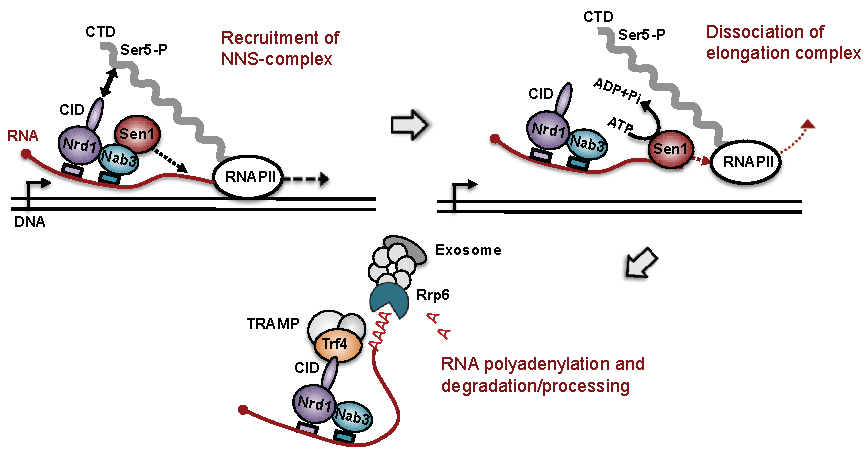
\includegraphics[width=\textwidth]{figures/introduction/nns}
\caption[Mechanism of NNS termination]{Main stages of NNS-dependent termination. the NNS complex is recruited thanks to \serf{}-phosphorylated CTD and sequence elements on the transcript. Termination is elicited by Sen1, presumably by translocating along the transcript. Finally, the exosome is recruited to the transcript and the transcript is either trimmed or completely degraded.}
\label{fig:nnsTermination}

\end{figure}


As previously mentioned, Nrd1 physically interacts with \gls{tramp}, and is responsible for the coordination between termination and 3' end processing.
The current model posits that when the Nrd1/Nab3 heterodimer is engaged with the Nascent RNA, Trf4 (and \gls{tramp}) can interact with Nrd1's \gls{cid}---either binding it directly, or displacing the \gls{ctd} of \gls{pol2} to get to it\cite{tudek:2014:molecular}.
After transcription termination has occurred, \gls{tramp} is thought to both recruit and stimulate the activity of the nuclear exosome.
How the exosome is recruited to \gls{tramp}---and therefore the transcript---is still unclear.
Recent studies have shown that \gls{tramp} is not the only effector of exosome recruitment, but that Nab3 can contact Rrp6 and bring the exosome to the RNA independently of \gls{tramp}.
\gls{tramp} stimulates the activity of the exosome via the addition of short poly(A) tails that are thought to provide an unstructured platform that can be easily threaded through the non-catalytic subunits of the ring. 
However, Air2 and Mtr4 are also thought to help deal with RNA secondary structure thanks to their RNA-binding and helicase activities.  
The exosome is known to act as a quality control step for short non-coding and aberrant transcripts.
It can, however, also act as in maturation of functional non-coding RNA (\gls{rrna}, \gls{sns}, and \gls{snos}) through trimming of their 3' ends to the appropriate length for their functional activities.

\subsection{Non-canonical termination pathways}

Despite \gls{cpf} and \gls{nns} being reliable mechanisms of transcription termination, presence of readthrough transcription that was not properly terminated is inevitable.
While readthrough constitutes less of a problem in metazoans---where the size of the genome allows polymerases to stray far from the termination site without impinging on other DNA-based biological processes---organisms with very compact genomes, such as \cer{}, have to deal with the possibility of transcriptional interference.

This phenomenon occurs when unterminated polymerases invade areas of the genome when other processes are taking place, disrupting them.
A simple example of transcriptional interference is represented in figure \ref{trInterference}\TODO{make figure for transcriptional interference}.
Because of the very small distance beween the termination site and the \gls{tss} of the following transcription unit, the polymerase is able to disrupt assembly of the \gls{pic}, resulting in severe downregulation of transcription initiation.

In order to protect these sensitive areas of the genome from stray polymerases, the cell has evolved several mechanisms of fail-safe transcription termination.
These mechanisms are non-canonical, as they usually emerge from already existing systems and are not dedicated solely to termination.
Nevertheless, several studies show wide-spread impact of these fail-safe termination mechanisms in preserving proper gene expression.

\subsubsection{Rnt1-dependent termination}

The yeast Rnase III homologue Rnt1 is an enzyme that binds and cleaves double-stranded RNA stem-loops. 
This activity serves as the first step in \gls{pol1} transcription termination \TODO{ref}.
After cleavage has occurred, unprotected 3' and 5' extremities can be attacked by exonucleases, leading to maturation of the transcript.

In the case of \gls{pol2} termination, Rnt1 is thought to act downstream of a subset of genes.
In case of \gls{cpf} failure in termination, transcription of an appropriate sequence element would create the right substrate for Rnt1.
After attacking and cleaving the stem-loop, the torpedo model of \gls{cpf} termination is thought to take over.
Rat1 would attack the newly formed 5' end and lead to termination through the mechanisms discussed in previous sections.
Although a similar termination mechanism was described in plants---where the protein Dcl4 is able to provide back-up termination at the FCA locus, know to possess a weak polyadenylation site---most mechanistic details regarding this termination mechanism remain unclear.

\subsubsection{Road-block termination}
  
Road-block termination represents another instance of non-canonical \gls{pol2} termination.
While established as a requisite for termination of \gls{pol1}, road-block has only very recently been demonstrated to be an \invivo{} mechanism for \gls{pol2} termination \cite{colin:2014:roadblock}.
In this study, the authors explored the role of the transcription factor Reb1 in limiting readthrough transcription.

Reb1 is an essential myb-like transcription factor that specifically and tightly binds the core sequence TTACCCG.
Binding to the sequence is highly specific, and mutation of one of the aforementioned nucleotides leads to almost complete abrogation of binding.
Reb1 sites are prevalent in promoter region and presence of this factor is linked to the recruitment of RSC complex\TODO{rsc acronym?}, known to displace nucleosome and generate \gls{nfr} at target promoters.

Reb1 sites were found to be associated with exosome-dependent transcripts whose 3' ends ended very precisely and abruptly 13-17 nucleotides from the Reb1 binding site. 
In addition, a prominent accumulation of \gls{pol2} was detected in the same region.
This pool of polymerases was shown to be pausing and a knock-out of TFIIS---preventing the resolution of backtracking (see section \ref{pausing})---resulted in increased \gls{pol2} occupancy in the proximity of reb1 sites.
\Invitro{} experiments showed that although Reb1 can act as a physical obstacle and cause \gls{pol2} to pause in its vicinity, this is not sufficient for termination and release of the polymerase from the template.
\Invivo{}, the molecular effector of termination was found to be the Rsp5/Elc1/Cul3 complex of ubiquitin ligases.
This complex is known for its activity in ubiquitinylating and degrading the larges subunit of \gls{pol2}, Rpb1\footnote{Also know as Rpo21}, when the polymerase is arrested because of DNA damage.

The current model for road-block termination posits that Reb1 prevents unterminated polymerases from invading nearby promoter regions. 
Reb1 acts as a physical obstacle that the polymerase cannot overcome, therefore, after several rounds of unsuccessful backtracking, the Rsp5/Elc1/Cul3 complex ubiquitinylates Rpb1, resulting in its proteasomal degradation and subsequent disassembly of the elongation complex.
The disassembly mediates the release of the transcript, which is polyadenylated by Trf4 and subsequently degraded by the exosome, although the mechanisms through which \gls{tramp} and the exosome are recruited is still unclear.

Given the compactness of the genome of \cer{}, the usefulness of this termination mechanism is immediately obvious. 
Promoters and potentially other sensitive regions of the genome can be protected from invading polymerase that could potentially disrupt other processes.
It remains unclear whether this mechanism has any counterpart in metazoans, where larger genomes make the problem of readthrough transcription less relevant.
Recent genome-wide experiments showed that accumulation of paused polymerases at certain transcription factor binding sites does occur in human.
However, whether this is linked to transcription termination remains to be elucidated \cite{mayer:2015:native}.

\clearpage